
\documentclass[10pt,mathserif]{beamer}

\usepackage{graphicx,amsmath,amssymb,tikz,psfrag}
\usepackage{pythonhighlight}

% ------------------------------------------------------------------------
% Packages
% ------------------------------------------------------------------------
\usepackage{amsmath}
\usepackage{tabularx}

% ------------------------------------------------------------------------
% Macros
% ------------------------------------------------------------------------
%~~~~~~~~~~~~~~~
% List shorthand
%~~~~~~~~~~~~~~~
\newcommand{\BIT}{\begin{itemize}}
\newcommand{\EIT}{\end{itemize}}
\newcommand{\BNUM}{\begin{enumerate}}
\newcommand{\ENUM}{\end{enumerate}}
%~~~~~~~~~~~~~~~
% Text with quads around it
%~~~~~~~~~~~~~~~
\newcommand{\qtext}[1]{\quad\text{#1}\quad}
%~~~~~~~~~~~~~~~
% Shorthand for math formatting
%~~~~~~~~~~~~~~~
\newcommand\mbb[1]{\mathbb{#1}}
\newcommand\mbf[1]{\mathbf{#1}}
\def\mc#1{\mathcal{#1}}
\def\mrm#1{\mathrm{#1}}
%~~~~~~~~~~~~~~~
% Common sets
%~~~~~~~~~~~~~~~
\def\reals{\mathbb{R}} % Real number symbol
\def\integers{\mathbb{Z}} % Integer symbol
\def\rationals{\mathbb{Q}} % Rational numbers
\def\naturals{\mathbb{N}} % Natural numbers
\def\complex{\mathbb{C}} % Complex numbers
\def\simplex{\mathcal{S}} % Simplex
%~~~~~~~~~~~~~~~
% Common functions
%~~~~~~~~~~~~~~~
\renewcommand{\exp}[1]{\operatorname{exp}\left(#1\right)} % Exponential
\def\indic#1{\mbb{I}\left({#1}\right)} % Indicator function
\providecommand{\maximize}{\mathop\mathrm{maximize}} % Defining math symbols
\providecommand{\minimize}{\mathop\mathrm{minimize}}
\providecommand{\argmax}{\mathop\mathrm{arg max}}
\providecommand{\argmin}{\mathop\mathrm{arg min}}
\providecommand{\arccos}{\mathop\mathrm{arccos}}
\providecommand{\asinh}{\mathop\mathrm{asinh}}
\providecommand{\dom}{\mathop\mathrm{dom}} % Domain
\providecommand{\range}{\mathop\mathrm{range}} % Range
\providecommand{\diag}{\mathop\mathrm{diag}}
\providecommand{\tr}{\mathop\mathrm{tr}}
\providecommand{\abs}{\mathop\mathrm{abs}}
\providecommand{\card}{\mathop\mathrm{card}}
\providecommand{\sign}{\mathop\mathrm{sign}}
\def\rank#1{\mathrm{rank}({#1})}
\def\supp#1{\mathrm{supp}({#1})}
%~~~~~~~~~~~~~~~
% Common probability symbols
%~~~~~~~~~~~~~~~
\def\E{\mathbb{E}} % Expectation symbol
\def\Earg#1{\E\left[{#1}\right]}
\def\Esubarg#1#2{\E_{#1}\left[{#2}\right]}
\def\P{\mathbb{P}} % Probability symbol
\def\Parg#1{\P\left({#1}\right)}
\def\Psubarg#1#2{\P_{#1}\left[{#2}\right]}
\def\Cov{\mrm{Cov}} % Covariance symbol
\def\Corr{\mrm{Corr}} % Covariance symbol
\def\Covarg#1{\Cov\left[{#1}\right]}
\def\Covsubarg#1#2{\Cov_{#1}\left[{#2}\right]}
\def\Corrsubarg#1#2{\Corr_{#1}\left[{#2}\right]}
\def\Var{\mrm{Var}}
\def\Vararg#1{\Var\left(#1\right)}
\def\Varsubarg#1#2{\Var_{#1}\left(#2\right)}
\newcommand{\family}{\mathcal{P}} % probability family
\newcommand{\eps}{\epsilon}
\def\absarg#1{\left|#1\right|}
\def\msarg#1{\left(#1\right)^{2}}
\def\logarg#1{\log\left(#1\right)}
%~~~~~~~~~~~~~~~
% Distributions
%~~~~~~~~~~~~~~~
\def\Gsn{\mathcal{N}}
\def\Ber{\textnormal{Ber}}
\def\Bin{\textnormal{Bin}}
\def\Unif{\textnormal{Unif}}
\def\Mult{\textnormal{Mult}}
\def\Cat{\textnormal{Cat}}
\def\Gam{\textnormal{Gam}}
\def\InvGam{\textnormal{InvGam}}
\def\NegMult{\textnormal{NegMult}}
\def\Dir{\textnormal{Dir}}
\def\Lap{\textnormal{Laplace}}
\def\Bet{\textnormal{Beta}}
\def\Poi{\textnormal{Poi}}
\def\HypGeo{\textnormal{HypGeo}}
\def\GEM{\textnormal{GEM}}
\def\BP{\textnormal{BP}}
\def\DP{\textnormal{DP}}
\def\BeP{\textnormal{BeP}}
%~~~~~~~~~~~~~~~
% Theorem-like environments
%~~~~~~~~~~~~~~~

%-----------------------
% Probability sets
%-----------------------
\newcommand{\X}{\mathcal{X}}
\newcommand{\Y}{\mathcal{Y}}
\newcommand{\D}{\mathcal{D}}
\newcommand{\Scal}{\mathcal{S}}
%-----------------------
% vector notation
%-----------------------
\newcommand{\bx}{\mathbf{x}}
\newcommand{\by}{\mathbf{y}}
\newcommand{\bt}{\mathbf{t}}
\newcommand{\xbar}{\overline{x}}
\newcommand{\Xbar}{\overline{X}}
\newcommand{\tolaw}{\xrightarrow{\mathcal{L}}}
\newcommand{\toprob}{\xrightarrow{\mathbb{P}}}
\newcommand{\laweq}{\overset{\mathcal{L}}{=}}
\newcommand{\F}{\mathcal{F}}


%% formatting

\mode<presentation>
{
\usetheme{default}
}
\setbeamertemplate{navigation symbols}{}
\usecolortheme[rgb={0.13,0.28,0.59}]{structure}
\setbeamertemplate{itemize subitem}{--}
\setbeamertemplate{frametitle} {
	\begin{center}
	  {\large\bf \insertframetitle}
	\end{center}
}

\newcommand\footlineon{
  \setbeamertemplate{footline} {
    \begin{beamercolorbox}[ht=2.5ex,dp=1.125ex,leftskip=.8cm,rightskip=.6cm]{structure}
      \footnotesize \insertsection
      \hfill
      {\insertframenumber}
    \end{beamercolorbox}
    \vskip 0.45cm
  }
}
\footlineon

\AtBeginSection[] 
{ 
	\begin{frame}<beamer> 
		\frametitle{Outline} 
		\tableofcontents[currentsection,currentsubsection] 
	\end{frame} 
} 

%% begin presentation

\title{\large \bfseries Bayesian Deep Learning}

\author{Kris Sankaran\\[3ex] Mila}

\date{\today}

\begin{document}
\maketitle

\section{Introduction}
\label{sec:introduction}

\begin{frame}
  \frametitle{Learning Objectives}
  \begin{itemize}
    \item Understand goals of deep learning, especially representation learning
    \item Logistic Regression to Backpropagation: Learn the modular-components
      view of deep learning
    \item Learn tricks for doing (and debugging) deep learning
    \item How to study deep learning algorithms: toy examples,
      drawing pictures, ...
  \end{itemize}
\end{frame}

\begin{frame}
  \frametitle{Flipping Coins}
  \begin{itemize}
  \item Likelihood function
  \item Entropy function
  \end{itemize} 
\end{frame}

\begin{frame}
  \frametitle{Using Data}
  \begin{itemize}
  \item What if the probability depended on input data?
  \end{itemize}
  \begin{figure}
    \centering
    \includegraphics[width=0.7\paperwidth]{figure/}
    \caption{Example of a classification problem, with a linear separation
      boundary. \label{fig:logistic_scatter} }
  \end{figure}
\end{frame}

\begin{frame}
  \frametitle{Using Data}
  \begin{itemize}
  \item What if the probability depended on input data?
  \end{itemize}
  \begin{figure}
    \centering
    \includegraphics[width=0.7\paperwidth]{figure/}
    \caption{Example with a nonlinear
      boundary. \label{fig:logistic_nonlinear_scatter} }
  \end{figure}
\end{frame}

\begin{frame}
  \frametitle{Updated Likelihood and Entropy}
  \begin{itemize}
  \item Likelihood
  \item Entropy
  \end{itemize}
  \begin{figure}
    \centering
    %% \includegraphics[width=0.7\paperwidth]{figure/}
    \caption{Updated likelihood and cross entropy functions if we want to
      incorporate $x$ information
      \label{fig:logistic_nonlinear_scatter} }
  \end{figure}
\end{frame}

\begin{frame}
  \frametitle{Logistic Regression}
  \begin{itemize}
  \item Logistic Regression $\rightarrow$ Finding good $\theta$'s for this
    likelihood
  \item Digression: When was logistic regression invented?
  \end{itemize}
\end{frame}

\begin{frame}
  \frametitle{Logistic Regression}
  \begin{itemize}
  \item Logistic Regression $\rightarrow$ Finding good $\theta$'s for this
    likelihood
  \item Digression: When was logistic regression invented?
  \end{itemize}
  \begin{figure}[ht]
    \centering
    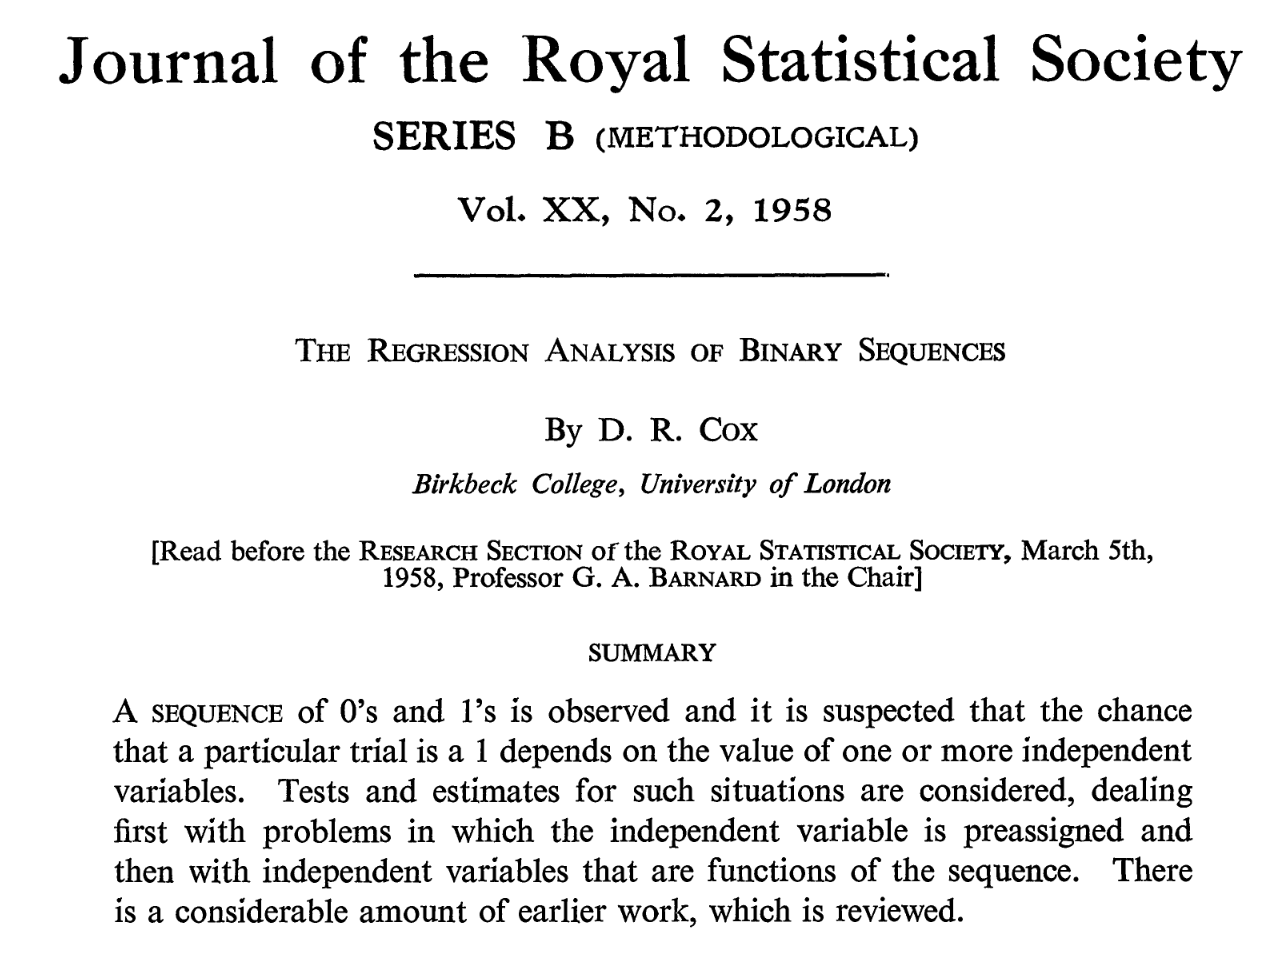
\includegraphics[width=0.4\paperwidth]{figure/logistic_paper}
    \caption{The inventor is still alive! \label{fig:logistic_paper} }
  \end{figure}
\end{frame}

\begin{frame}
  \frametitle{Logistic Regression}
  \begin{itemize}
  \item Logistic Regression $\rightarrow$ Finding good $\theta$'s for this
    likelihood
  \item Digression: When was logistic regression invented?
  \end{itemize}
  \begin{figure}[ht]
    \centering
    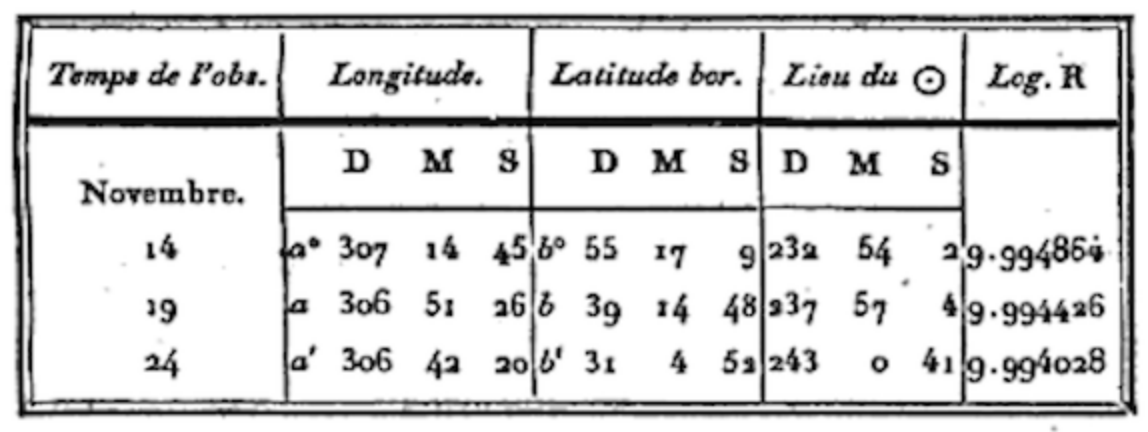
\includegraphics[width=0.7\paperwidth]{figure/least_squares}
    \caption{First public demonstration of least squares (Legendre,
      1805). \label{fig:least_squares} }
  \end{figure}
\end{frame}

\begin{frame}
  \frametitle{Optimization}
\end{frame}

\begin{frame}
  \frametitle{Review: The Chain Rule}
\end{frame}

\begin{frame}
  \frametitle{Chain Rule for Logistic Regression}
\end{frame}

\section{Representation Learning}

\begin{frame}
  \frametitle{Finding Meaningful Features}
 \begin{itemize}
 \item What if our $x_i$'s are unstructured?
 \item Logistic regression only succeeds when raw input coordinates are
   meaningful
 \end{itemize} 
 \begin{figure}[ht]
   \centering
   \includegraphics[width=0.7\paperwidth]{figure/image_features}
   \caption{It would be nice if our images came with qualitative annotation
     about what was in them. \label{fig:image_features} }
 \end{figure}
\end{frame}

\begin{frame}
  \frametitle{Finding Meaningful Features}
 \begin{itemize}
 \item What if our $x_i$'s are unstructured?
 \item Logistic regression only succeeds when raw input coordinates are
   meaningful
 \end{itemize} 
 \begin{figure}[ht]
   \centering
   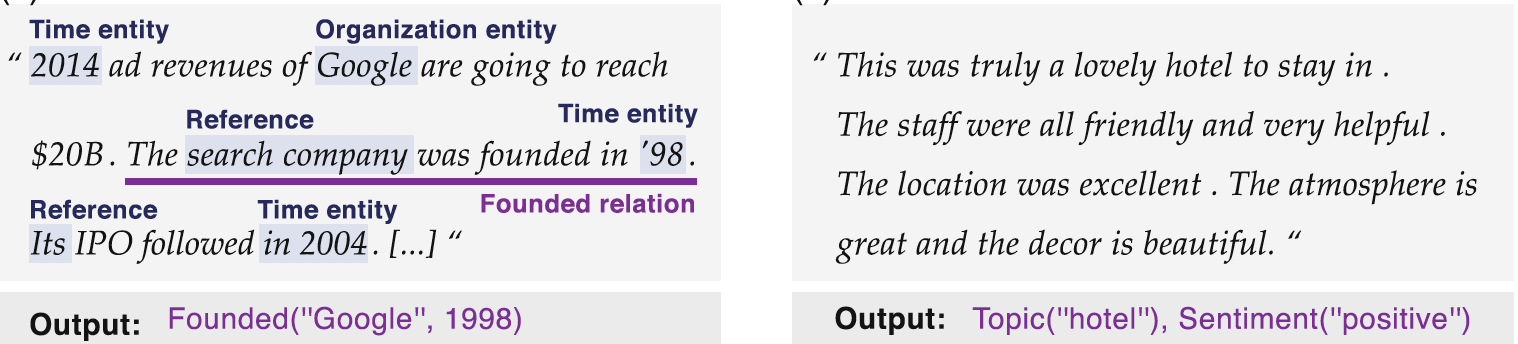
\includegraphics[width=0.7\paperwidth]{figure/language_features}
   \caption{Similarly, extracting meaningful structure from raw text would be
     useful in a variety of downstream tasks. \label{fig:language_features} }
 \end{figure}
\end{frame}

\begin{frame}
  \frametitle{Our Goal}
\end{frame}

\begin{frame}
  \frametitle{Stacking Logistic Regressions}
  \begin{itemize}
  \item Idea: Let logistic regression learn the features that help it classify
    well
  \item To do this, allow nonlinear transformations leading to final
    classification layer
  \item Successive layers learn more complex feature representations
  \end{itemize}
  \begin{figure}
      \centering
      \includegraphics[width=0.7\paperwidth]{figure/stacked_logistic}
      \caption{The basic idea of deep learning is to stack many logistic
        regression layers. \label{fig:stacked_logistic} }
\end{figure}
\end{frame}

\begin{frame}
  \frametitle{Aside: Can't Stack Linear Regressions}
  \begin{itemize}
  \item Multiple linear layers $\rightarrow$ function still linear
  \item Wouldn't be any richer than ordinary linear regression
  \end{itemize} 

\end{frame}

\begin{frame}
  \frametitle{Aside: Activations}
  \begin{itemize}
  \item For nonlinearity, we used sigmoid
  \item Many types of nonlinearities can be used instead
  \item Most common these days are Rectified Lienar Unites (ReLUs)
    \begin{itemize}
    \item They are easier to optimize (alleviate vanishing gradient problem)
    \end{itemize}
  \end{itemize} 
\end{frame}

\begin{frame}
  \frametitle{Optimization: Stochastic Gradient Descent}
  \begin{itemize}
  \item Optimize parameters by moving in a direction expected to decrease
    overall loss
  \item SGD: Expected direction of overall gradient, after looking at small
    batch of data
  \item These days, other methods used too -- Adam, AdaGrad, AdaDelta, ...
  \end{itemize}
\end{frame}

\begin{frame}
  \frametitle{Dynamic Programming view of Backpropagation}
  \begin{itemize}
  \item For each iteration of SGD, we need to estimate the gradient of the loss
    with respect to the parameters
  \item Cost can be reduced by noticing computation of derivatives for lower
    layers can make use of gradients from higher layers
  \end{itemize}
  \begin{figure}
    \centering
    %% \includegraphics[width=0.7\paperwidth]{figures/backprop_diagram}
    \caption{\label{fig:backprop_diagram} }
  \end{figure}
\end{frame}

\begin{frame}
  \frametitle{Modularity}
  \begin{itemize}
  \item Gradients make use only of \textit{local} information
  \item Can propose arbitrary new layers, as long as you can define gradient of
    output with respect to input
  \item Has let people experiment widely in literature,
    \begin{itemize}
    \item Convolution layers
    \item Attention mechanisms
    \item LSTM cells
    \item ...
    \end{itemize}
  \end{itemize} 
\end{frame}

\section{Types of Layers}

\begin{frame}
  \frametitle{Fully Connected}
\begin{figure}
  \centering
  \includegraphics[width=0.7\paperwidth]{figures/fully_connected_vis}
  \caption{All the outputs from one layer can affect all the inputs to the next
    one. \label{fig:fully_connected}}
\end{figure}
\end{frame}

\begin{frame}
  \frametitle{Fully Connected (Math)}
\end{frame}

\begin{frame}
  \frametitle{Convolution + Pooling}
  \begin{figure}
    \centering
    \includegraphics[width=0.7\paperwidth]{figures/convolutional_vis}
    \caption{Convolution compares small patches against prespecified
      ``filters.'' Since it uses the same filters for all patches, the number of
      parameters is greatly reduced.
       \label{fig:convolutional_vis}}
  \end{figure}
\end{frame}

\begin{frame}
  \frametitle{Residual Layer}
  \begin{figure}[
      \centering
      \includegraphics[width=0.7\paperwidth]{figure/resnet_vis}
      \caption{Residual Networks use layers to incrementally 
        add complexity, by directly copying the previous values and only
        learning minor modifications on top of that. \label{fig:resnet_vis} }
  \end{figure}
\end{frame}

\begin{frame}
  \frametitle{Residual Layer (Math)}
\end{frame}

\begin{frame}
  \frametitle{Attention Mechanisms}
\end{frame}

\begin{frame}
  \frametitle{Gated Recurrent Units}
\end{frame}

\section{Debugging Deep Learning}

\begin{frame}
  \frametitle{Hyperparameter Tuning}
  \begin{itemize}
  \item Deep learning models can be hard to train
  \item Depending on various hyperparameters,
    \begin{itemize}
    \item Sequence of (per-layer) learning rates
    \item Weight initialization
    \item Type, number, and width of each layer
    \item Activation functions
    \end{itemize}
    the model may or may not train properly
  \end{itemize}
\end{frame}

\begin{frame}
  \frametitle{Training Analysis}
  \begin{figure}[ht]
    \centering
    %% \includegraphics[width=0.7\paperwidth]{figure/}
    \caption{Typical strategy is to try to first overfit the model, then
      regularize to ensure validation performance. \label{fig:learning_curves} }
  \end{figure}
\end{frame}

\begin{frame}
  \frametitle{Training Analysis}
  \begin{itemize}
  \item It can be helpful to collect statistics
    \begin{itemize}
    \item Gradients
    \item Activation values
    \end{itemize}
  \item Save your model at checkpoints! Helps both debugging and restarting
    training
  \end{itemize}
\end{frame}

\begin{frame}
  \frametitle{Final Remarks}
  
\end{frame}

  %% \begin{figure}
  %%   \centering
  %%   \includegraphics[width=0.7\paperwidth]{figure/}
  %%   \caption{\label{fig:coin_flipping_data} }
  %% \end{figure}
\end{document}
